

\tikzset{every picture/.style={line width=0.75pt}} %set default line width to 0.75pt        

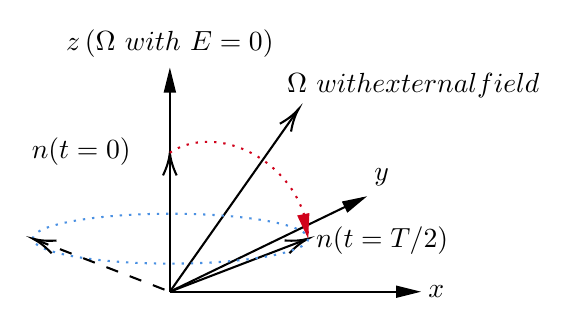
\begin{tikzpicture}[x=0.75pt,y=0.75pt,yscale=-1,xscale=1]
%uncomment if require: \path (0,300); %set diagram left start at 0, and has height of 300

%Straight Lines [id:da8125477960653353] 
\draw    (95,171) -- (214,171) ;
\draw [shift={(216,171)}, rotate = 180] [fill={rgb, 255:red, 0; green, 0; blue, 0 }  ][line width=0.08]  [draw opacity=0] (12,-3) -- (0,0) -- (12,3) -- cycle    ;
%Straight Lines [id:da5838070816593157] 
\draw    (95,171) -- (95,65.02) ;
\draw [shift={(95,63.02)}, rotate = 450] [fill={rgb, 255:red, 0; green, 0; blue, 0 }  ][line width=0.08]  [draw opacity=0] (12,-3) -- (0,0) -- (12,3) -- cycle    ;
%Straight Lines [id:da8598243285485796] 
\draw    (95,171) -- (188.2,125.89) ;
\draw [shift={(190,125.02)}, rotate = 514.1700000000001] [fill={rgb, 255:red, 0; green, 0; blue, 0 }  ][line width=0.08]  [draw opacity=0] (12,-3) -- (0,0) -- (12,3) -- cycle    ;
%Straight Lines [id:da43220335567629653] 
\draw    (95,171) -- (155.85,84.66) ;
\draw [shift={(157,83.02)}, rotate = 485.17] [color={rgb, 255:red, 0; green, 0; blue, 0 }  ][line width=0.75]    (10.93,-3.29) .. controls (6.95,-1.4) and (3.31,-0.3) .. (0,0) .. controls (3.31,0.3) and (6.95,1.4) .. (10.93,3.29)   ;
%Straight Lines [id:da7003435646275242] 
\draw    (95,106.02) -- (95,171) ;
\draw [shift={(95,104.02)}, rotate = 90] [color={rgb, 255:red, 0; green, 0; blue, 0 }  ][line width=0.75]    (10.93,-3.29) .. controls (6.95,-1.4) and (3.31,-0.3) .. (0,0) .. controls (3.31,0.3) and (6.95,1.4) .. (10.93,3.29)   ;
%Shape: Arc [id:dp7751197002401395] 
\draw  [draw opacity=0][dash pattern={on 0.84pt off 2.51pt}] (95,104.02) .. controls (108.77,94.84) and (129.93,97.81) .. (145.49,112.08) .. controls (155.82,121.57) and (161.4,133.95) .. (161.64,145.45) -- (121.82,137.87) -- cycle ; \draw  [color={rgb, 255:red, 208; green, 2; blue, 27 }  ,draw opacity=1 ][dash pattern={on 0.84pt off 2.51pt}] (95,104.02) .. controls (108.77,94.84) and (129.93,97.81) .. (145.49,112.08) .. controls (155.82,121.57) and (161.4,133.95) .. (161.64,145.45) ;
%Straight Lines [id:da9547032756267608] 
\draw    (159.77,146.16) -- (95,171) ;
\draw [shift={(161.64,145.45)}, rotate = 159.02] [color={rgb, 255:red, 0; green, 0; blue, 0 }  ][line width=0.75]    (10.93,-3.29) .. controls (6.95,-1.4) and (3.31,-0.3) .. (0,0) .. controls (3.31,0.3) and (6.95,1.4) .. (10.93,3.29)   ;
%Straight Lines [id:da44322203840446583] 
\draw [color={rgb, 255:red, 208; green, 2; blue, 27 }  ,draw opacity=1 ]   (160.64,140.45) -- (161.25,143.48) ;
\draw [shift={(161.64,145.45)}, rotate = 258.69] [fill={rgb, 255:red, 208; green, 2; blue, 27 }  ,fill opacity=1 ][line width=0.08]  [draw opacity=0] (12,-3) -- (0,0) -- (12,3) -- cycle    ;
%Shape: Ellipse [id:dp5189226557816553] 
\draw  [color={rgb, 255:red, 74; green, 144; blue, 226 }  ,draw opacity=1 ][dash pattern={on 0.84pt off 2.51pt}] (29,145.45) .. controls (29,138.81) and (58.69,133.43) .. (95.32,133.43) .. controls (131.95,133.43) and (161.64,138.81) .. (161.64,145.45) .. controls (161.64,152.08) and (131.95,157.46) .. (95.32,157.46) .. controls (58.69,157.46) and (29,152.08) .. (29,145.45) -- cycle ;
%Straight Lines [id:da5564344266734615] 
\draw  [dash pattern={on 4.5pt off 4.5pt}]  (30.87,146.17) -- (95,171) ;
\draw [shift={(29,145.45)}, rotate = 21.17] [color={rgb, 255:red, 0; green, 0; blue, 0 }  ][line width=0.75]    (10.93,-3.29) .. controls (6.95,-1.4) and (3.31,-0.3) .. (0,0) .. controls (3.31,0.3) and (6.95,1.4) .. (10.93,3.29)   ;

% Text Node
\draw (218,171) node [anchor=west] [inner sep=0.75pt]    {$x$};
% Text Node
\draw (95,59.62) node [anchor=south] [inner sep=0.75pt]    {$z\left(\boldsymbol{\Omega } \ \text{with} \ \boldsymbol{E} =0\right)$};
% Text Node
\draw (192,121.62) node [anchor=south west] [inner sep=0.75pt]    {$y$};
% Text Node
\draw (150,64.4) node [anchor=north west][inner sep=0.75pt]    {$\boldsymbol{\Omega } \ \text{with external field}$};
% Text Node
\draw (27,95.4) node [anchor=north west][inner sep=0.75pt]    {$\boldsymbol{n}( t=0)$};
% Text Node
\draw (164,138.4) node [anchor=north west][inner sep=0.75pt]    {$\boldsymbol{n}( t=T/2)$};


\end{tikzpicture}
